\documentclass{article}
\usepackage{amsmath}
\usepackage[utf8]{inputenc}
\usepackage{graphicx}
\usepackage{enumerate}
\usepackage{pgfplots}
\pgfplotsset{compat=1.12}
\setlength{\parskip}{\baselineskip}%
\setlength{\parindent}{0pt}%

\begin{document}
\begin{titlepage}
\title{Lösning Veckotest 3, MA1439}
\author{Henrik Samuelsson}
\maketitle
\thispagestyle{empty}
\end{titlepage}

\section*{Uppgift 1.}
Lös andragradsekvationerna
\begin{enumerate}[(a)]
\item $x^2+8x+7=0$
\item $x(x+23)=0$
\item $2x^2-8x-10=0$
\end{enumerate}

\textbf{Lösning}
\begin{enumerate}[(a)]
\item
$x=-\dfrac{8}{2}\pm\sqrt{\left(\dfrac{8}{2}\right)^2-7}=-4\pm\sqrt{16-7}=-4\pm3$

$x_1 = -1$

$x_2 = -7$

\item
Om en produkt av två faktorer är $0$ så måste minst en av faktorerna vara noll. Detta ger direkt lösningen

$x_1 = 0$

$x_2 = -23$

\item
Dela båda sidor med $2$

$\dfrac{2x^2-8x-10}{2}=\dfrac{0}{2}$

$x^2-4x-5 = 0$

Ekvationen är nu på den form som vi behöver för kunna använda den kända formeln för andragradsekvationer

$x=\dfrac{4}{2}\pm\sqrt{\left(\dfrac{4}{2}\right)^2+5}=2\pm\sqrt{4+5}=2\pm3$

$x_1 = 5$

$x_2 = -1$
\end{enumerate}

\section*{Uppgift 2.}
\begin{enumerate}[(a)]
\item Bestäm eventuella nollställen till funktionen $f(x)=x^2-x+1$.
\item Skissa grafen.
\end{enumerate}

\begin{enumerate}[(a)]
\item 
Eventuella nollställen hittas genom att sätta $f(x)$ till $0$

$x^2-x+1=0$

Vi använder lösningsformeln för andragradsekvationer.

$x=-\dfrac{1}{2}\pm\sqrt{\dfrac{1}{2}^2-1}=-\dfrac{1}{2}\pm\sqrt{-\dfrac{3}{4}}$

Ekvationen saknar reella rötter vilket betyder att den givna funktionen saknar nollställen.

\item Grafen för funktionen kan ses i figuren nedan.

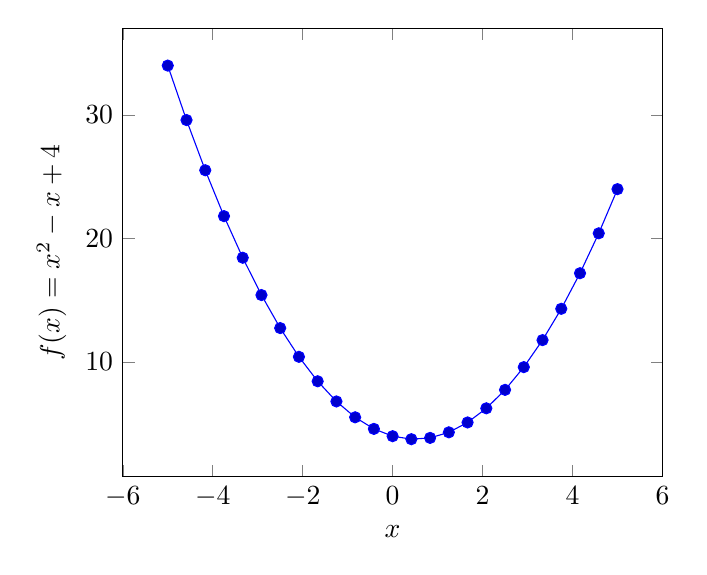
\begin{tikzpicture}
	\begin{axis}[
		xlabel=$x$,
		ylabel={$f(x) = x^2 - x +4$}
	]
	% use TeX as calculator:
	\addplot {x^2 - x +4};
	\end{axis}
\end{tikzpicture}

\end{enumerate}

\section*{Uppgift 3.}
Lös rotekvationerna
\begin{enumerate}[(a)]
\item $\sqrt{x+5}=3+x$
\item $\sqrt{3x+4})=8-x$
\end{enumerate}

\textbf{Lösning}

Denna typ av uppgift kan lösas genom att först kvadrera båda sidor och sedan använda lösningsformeln för andragradsekvationer.

\begin{enumerate}[(a)]
\item
$\sqrt{x+5}=3+x$

$x+5=(3+x)^2$

$x+5=9+6x+x^2$

$x^2+5x+4=0$

$x=-\dfrac{5}{2}\pm\sqrt{\left(\dfrac{5}{2}\right)^2-4}=-2,5\pm\sqrt{\dfrac{9}{4}}=-2,5\pm1,5$

$x_1 = -1$

$x_2 = -4$

Vi har två rötter kontroll genom insättning i ursprungsekvationen visar att $x_2$ är en så kallad falsk rot.

Svaret på uppgiften är 

$x = -1$

\item
$\sqrt{3x+4}=8-x$

$3x+4=(8-x)^2$

$3x+4=64-16x+x^2$

$x^2-19x+60=0$

$x=\dfrac{19}{2}\pm\sqrt{\left(\dfrac{19}{2}\right)^2-60}=\dfrac{19}{2}\pm\sqrt{\dfrac{121}{4}}=\dfrac{19}{2}\pm\dfrac{11}{2}$

$x_1 = 15$

$x_2 = 4$

Vi har två rötter kontroll genom insättning i ursprungsekvationen visar att $x_1$ är så kallad falsk rot.

Svaret på uppgiften är 

$x = 4$
\end{enumerate}

\section*{Uppgift 4.}
Bestäm koordinaterna för följande funktions största eller minsta värde (vertex)

$f(x)=10x-x^2-21$

\textbf{Lösning}

Eftersom $x^2$ termen är negativ så kommer vertex vara vid funktionens största värde. Lutningen av funktionens graf kommer att vara $0$ i vertex. Genom att derivera så får vi fram lutningen

$f'(x)=10-2x$

$0=10-2x$

$x=5$

Vi vet nu x-koordinaten, sätt in detta värde i funktionen för att få fram y-koordinaten

$f(5)=10\cdot5-5^2-21=4$

Alltså så har funktionen ett största värde i punkten $(5,4)$

\end{document}
